%\setcounter{chapter}{-1}
\chapter{Uncertainty in Complex Systems: The Role of Fuzzy Logic}
\label{ch:intro}


Before stating a proper formalization of the fuzzy framework, it is crucial to first clarify what it represents and why there is a need for such a theory when there already exists Probability and Statistics, which are broadly applied and much more developed.\\

The main objective of these frameworks is to represent and manage uncertainty inherent in complex systems. This involves encoding data and expressing information through appropriate mathematical structures and developing measures that enable effective synthesis and combination of uncertain information.\\

A fundamental motivation for modeling uncertainty is to enable better decision making across diverse domains. In engineering, uncertainty quantification helps assess structural reliability and optimize designs. In finance, it aids risk management and portfolio optimization. In medicine, it supports diagnosis and treatment planning under incomplete information. In environmental science, it helps model climate patterns and ecological systems. By developing mathematical frameworks to represent and reason about uncertainty, we can make more informed choices and balance competing objectives in complex scenarios.\\

\section{Uncertainty: Definition and Types}

There is no consensus about a unique definition of uncertainty and a single classification of its types. 

As mentioned above, uncertainty is present in complex systems. According to \cite{UncertaintySciences}, \textbf{systems are abstractions that aid understanding} a group of interacting, interrelated, or interdependent elements that together form a complex whole, which can be a physical structure, process, or procedure with some attributes of interest. All parts of a system are related to the same overall process, procedure, or structure. \\

Notice that usually these abstractions are not unique in the sense that there are different ways to model the same system. Formally it is:

\begin{definition}[System]
    An object is called a system if it can be expressed as a pair of a set of things ($T$) and a set of relations ($R$).

    \[S = (T,R)\]
\end{definition}

\begin{remark}
    By \emph{set of things}, we mean that \(T\) may be any collection of elements, from a simple set (finite or infinite) to more complex structures such as sets of sets or power sets. Likewise, the \emph{set of relations} (\(R\)) is understood broadly, it encapsulates interactions, constraints, and dependencies between these elements; providing a structural foundation. Hence, even though \((T, R)\) appears simple, its components can be very varied and rich.
\end{remark}

This definition is too general to have any practical utility. However, it gives us a flexible ''skeleton" to build upon and tackle what we refer to with \textit{uncertainty in a system}. \\

Finding a proper definition for uncertainty is a very subtle and challenging task due to the ample scope of the concept, but following the ideas from \cite{UncertaintySciences} and \cite{RumsfeldMatrix} we will start by classifying knowledge into 4 categories using Rumsfeld's Matrix\footnote{While \cite{RumsfeldMatrix} classifies this matrix as representing only epistemic uncertainty, we take a broader view since aleatoric uncertainty, with its quantifiable regularities through probability distributions, can be considered a ''known unknown".}:

\begin{table}[h!]
    \centering
    \label{tab:rumsfeld}
    \begin{tabular}{@{}c@{~}c|c|c|}
        \multicolumn{2}{c}{} & \multicolumn{2}{c}{\large \textbf{Our Perceived Knowledge}} \\[0.3em]
        \multicolumn{2}{c}{} & \multicolumn{1}{c}{Known} & \multicolumn{1}{c}{Unknown} \\
        \cline{3-4}
        \multirow{2}{*}{\rotatebox{90}{\parbox{2cm}{\centering \large \textbf{Real State of} \\ \textbf{Knowledge}}}} 
        & Known & Things we know we know & Things we know we don't know \\
        \cline{3-4}
        & Unknown & Things we do not know we know & Things we do not know we don't know \\
        \cline{3-4}
    \end{tabular}
    \vspace{1cm}
    \caption{Rumsfeld's Matrix}
\end{table}

This matrix illustrates the relationship between knowledge and ignorance\footnote{For a more rigorous treatment of ignorance and higher-order ignorance using non-formal modal logic see \cite{firstorderignorance}.}, where ignorance can be understood as the absence or incompleteness of knowledge. In particular, we would consider \textbf{ignorance} to be represented in the \textit{Unknown} column and \textbf{knowledge}, in the \textit{Known} column. From this perspective, we can identify:
% \begin{itemize}
%     \item \textbf{Known Knowns}: things we are aware of and understand well.
%     \item \textbf{Unknown Knowns}: these are the aspects that we actually know but are not conciously aware of. They might include tacit knowledge or assumptions that go unrecognized.
%     \item \textbf{Known Unknowns}: gaps in our knowledge that we recognize.
%     \item \textbf{Unknown Unknowns}: things we are completely unaware of.
% \end{itemize}
 
\begin{tikzpicture}[remember picture, every node/.style={anchor=west}]
    % First group: Knowledge
    \node (knowledge) at (0,0) {%
      \begin{minipage}{0.8\textwidth}
        \begin{itemize}[leftmargin=1cm]
          \item \textbf{Known Knowns}: things we are aware of and understand well.
          \item \textbf{Unknown Knowns}: these are the aspects that we actually know but are not consciously aware of.
        \end{itemize}
      \end{minipage}%
    };
    
    % Second group: Ignorance
    % Increase vertical gap below ''knowledge" to avoid overlap
    \node (ignorance) [below=0.5cm of knowledge] {%
      \begin{minipage}{0.8\textwidth}
        \begin{itemize}[leftmargin=1cm]
          \item \textbf{Known Unknowns}: gaps in our knowledge that we recognize.
          \item \textbf{Unknown Unknowns}: things we are completely unaware of.
        \end{itemize}
      \end{minipage}%
    };
    
    % Draw curly brace for Knowledge
    % Shift it further left (xshift=-1.2cm) and move label out (xshift=-0.6cm)
    \draw[
      decorate,
      decoration={brace, amplitude=10pt, mirror}
    ] 
      ([xshift=0.6cm]knowledge.north west) 
      -- 
      ([xshift=0.6cm]knowledge.south west)
      node[midway, left, xshift=-0.6cm,yshift=1cm, rotate=90] {\large Knowledge};
    
    % Draw curly brace for Ignorance
    \draw[
      decorate,
      decoration={brace, amplitude=10pt, mirror}
    ] 
      ([xshift=0.6cm]ignorance.north west) 
      -- 
      ([xshift=0.6cm]ignorance.south west)
      node[midway, left, xshift=-0.6cm,yshift=1cm, rotate=90] {\large Ignorance};
  \end{tikzpicture}

In the context of uncertainty quantification, we focus primarily on the \textbf{known unknowns} because those are the aspects of ignorance that can be identified and attempted to model. With this idea in mind, we can finally state what we will consider as uncertainty in this work:\\


\begin{definition}[Uncertainty in a system]
    \say{The term uncertainty can be viewed as \textbf{a component of ignorance}.[...] Uncertainty and information as a pair, and ignorance and knowledge as another pair,[...], as the former component of each pair describes a deficiency in the respective latter component, while the latter component of a pair can be viewed as the respective capacity available to reduce the respective former component.}\cite{UncertaintySciences}
\end{definition}

It is useful to classify different types of uncertainty to better understand what our mathematical models represent. However, it is vital to keep in mind that these types are not independent of each other. Rather than strict boundaries where every known unknown fits, it is better to think of them as dimensions of uncertainty. The most broadly used classification of uncertainty is this binary one:\\

\begin{itemize}
    \item \textbf{Aleatoric:} inherent randomness or natural variability, which is \textbf{irreducible}. This is the most familiar one to the general public since it is the one that appears in the famous example of throwing a fair dice, and it is a case of success of probability theory.
    \item \textbf{Epistemic Uncertainty}: arises from incomplete knowledge, measurement limitations, imperfect models, or lack of data. This uncertainty \textbf{may be reducible} if additional information or resources become available. 
    %Some examples include: 
    % \begin{itemize} 
    %     \item Estimating voter preferences from a poll of 10 people involves high epistemic uncertainty; polling 10,000 voters significantly reduces this uncertainty, providing a clearer representation of true preferences. 
    %     \item Imagine a sensor that detects if a temperature is above a threshold. Even if we have 2 objects at different temperature above that level, we would need to group them together. This situation presents uncertainty due to the limited granularity of our knowledge, known as \textbf{coarseness} (which is a type of epistemic uncertainty).
    % \end{itemize} 
\end{itemize}

Nevertheless, this binary classification has several important limitations:

\begin{itemize}
    \item \textbf{Incomplete Coverage:} Some forms of uncertainty do not neatly fit into these two categories. For example: vagueness, which is not aleatoric but neither reducible with more data.
    \item \textbf{Fail to capture higher-order uncertainties:} does not account for meta-uncertainties (uncertainty about the uncertainty itself) or a broader hierarchical nature of ignorance.
    \item \textbf{Interdependence Oversight:} The influence between each other is not taken into account.
\end{itemize}

% A classification of uncertainty types allow us to build a proper representation tailored to a specific kind of ignorance. 
Given these limitations of the binary classification, we will adopt a more nuanced framework based on \cite{UncertaintySciences}. While their full classification system is more extensive than needed for our purposes, here it is presented a simplified version that better captures the complexity of uncertainty while remaining practical for our analysis. Another important remark is that while specific frameworks are associated with each type of uncertainty (even the same framework with multiple uncertainty types), alternative modeling approaches exist and can be effectively used.


\begin{itemize}
    \item \textbf{Nonspecificity:} Uncertainty resulting from insufficient specificity or detail, information is insufficient to precisely specify which outcome or event applies. 
    \begin{itemize}
        \item \textit{Example:} Knowing only that the solution to an equation lies within a set \(\{1, 2, 3\}\), but without further precision.
        \item \textit{Frameworks:} Modeled primarily by crisp set theory and possibility theory, where uncertainty arises from ambiguous specification of possibilities. For example, this is what is modeled when assigning a domain for a random experiment.
    \end{itemize}

    \item \textbf{Vagueness:} Arises from imprecise, unclear, or fuzzy boundaries in concepts, meaning that elements can partially belong to a category. 
    \begin{itemize}
        \item \textit{Example:} Categorizing a temperature as ''hot"; the boundary between hot and not-hot is not clearly defined; it is not crisp.
        \item \textit{Frameworks:} Modeled using fuzzy set theory, assigning partial membership values between 0 and 1 to indicate degrees of compatibility between elements and sets.
    \end{itemize}

    \item \textbf{Coarseness (Granularity):} Uncertainty due to limited resolution in the available data or knowledge, making it difficult to distinguish precisely between similar elements.
    \begin{itemize}
        \item \textit{Example:} A doctor has patient records with temperatures and cough symptoms, but can only match new patients' temperatures with cough symptoms at a coarse level (e.g. 37.3°C and 37.4°C are treated as identical since the records don't include every possible temperature value), limiting the precision of symptom prediction.
        \item \textit{Frameworks:} Modeled using rough set theory, i.e. equivalence classes to define lower and upper approximations of a set to manage indistinguishability caused by granularity.
    \end{itemize}

    \item \textbf{Randomness (Aleatoric Uncertainty):} Intrinsic uncertainty in stochastic processes, inherently irreducible, even with complete knowledge of the system.
    \begin{itemize}
        \item \textit{Example:} Predicting the outcome of a fair dice roll.
        \item \textit{Frameworks:} Modeled by probability theory through probability distributions, which represent expected frequencies in repeated experiments but unable to deterministically predict individual outcomes.
    \end{itemize}

    \item \textbf{Epistemic Uncertainty:} Uncertainty arising from incomplete understanding of the true structure, parameters, or mechanisms governing a system. This can include potentially missing or incorrect model assumptions. It is often considered reducible through targeted investigations, refining model assumptions, or incorporating more informative data expanding the knowledge of the underlying system.

    \begin{itemize}
        \item \textit{Example:} Modeling a physical process but without knowing whether it is linear or nonlinear; further experiments could reveal the correct functional form.
        \item \textit{Frameworks:} Often modeled via Bayesian inference (updating priors with data), possibility theory, belief functions, and interval methods. The focus is on refining or correcting a model (e.g., identifying correct distributions, dependencies, causal structures).
    \end{itemize}

    \item \textbf{Sampling Uncertainty:} Uncertainty emerging from inferring properties of a population based solely on a limited sample from it. This uncertainty decreases as the sample size approaches the population size.
    \begin{itemize}
        \item \textit{Example:} Estimating the average height of a country's population from measurements of a random subset. 
        \item \textit{Frameworks:} Modeled by inferential statistics, confidence intervals, hypothesis testing, and conformal prediction methods, explicitly quantifying the variability and uncertainty in such inferences.
    \end{itemize}
\end{itemize}

A final consideration worth discussing is \textbf{the distinction between subjectivity and objectivity in uncertainty representation}. 
This distinction plays an important role in frameworks like Bayesian statistics (through the specification of prior distributions) and is particularly relevant in fuzzy set theory where membership values often reflect a decision maker's subjective assessment. However, while the source of uncertainty may differ (subjective judgment versus objective measurement), we will treat them as formally equivalent in their mathematical representation. The only practical distinction may arise when decision makers assign importance weights, potentially weighting objective and subjective sources differently according to their preferences.\\

The boundary between what may be considered objective versus subjective in fuzzy sets is often unclear. Consider this illustrative example that highlights this ambiguity:
Suppose we want to determine the membership degree of a person who is 180cm tall to the set of ''tall people". One approach would be to assign a value based on personal perception, a subjective assessment influenced by our own height, the heights of people we know, and even potentially varying over time as our perception changes. Alternatively, we could use the population height percentile as the membership degree, which seems more objective. However, this choice still involves subjective decisions: for instance, why use the percentile directly rather than its square root?\\

\section{Vagueness and Sorites Paradox}
\label{sec:sorites}

Among the uncertainty types discussed above, vagueness is most relevant to the following chapters, as it is mainly modeled using fuzzy sets.\\

Fuzzy sets extend classical sets by introducing partial memberships, moving beyond the binary notion of ``belongs" or ``does not belong". This provides a more expressive framework for modeling concepts that cannot be adequately represented using traditional sets.\\

To demonstrate the necessity of fuzzy sets and following \cite{HájekSorites}, let us consider the Sorites Paradox. Attributed to the philosopher Eubulides, this paradox emerges from the following type of reasoning:

\begin{enumerate}
    \item A single grain of sand does not form a heap.
    \item Adding one grain to something that is not a heap does not make it a heap.
    \item Consequently, there are no heaps.
\end{enumerate}


There are many variations of this paradox with different vague concepts such as age, size, height, baldness, etc. All share the same issue: there is a gradual transition, and evaluating to only true or false does not allow us to represent it adequately, therefore reaching a contradiction.\\

This paradox can be resolved by considering partial membership to the set of heaps, where a single grain may have 0.001 membership which grows with the number of grains until reaching a group of a million grains, which could have 1 membership. While these numbers are arbitrary, this model better captures our intuitive concept of a heap than the conclusion that ``heaps do not exist".\\

An important remark is that Sorites paradox is originally formulated in terms of truth values rather than set memberships. Nevertheless, it is natural to assume a direct relationship between the degree of membership of a given amount of grains to the set of heaps and the truth value of the proposition \textit{``This amount of grains is a heap"}. In the paper \cite{HájekSorites}, the authors argue that the proposition ``\textit{Adding one grain to something that is not a heap does not make it a heap}" is not strictly true but rather almost true, thus by considering varying degrees of truth we avoid the contradiction.\\

This example illustrates how vagueness is the core issue with these concepts: the boundary of the set of heaps is not crisp but rather fuzzy. There is no precise point where something transitions from not being a heap to being one, it is a gradual process. \\

In the following chapters, we will demonstrate that fuzzy logic and the treatment of vagueness is not merely an academic curiosity, but rather a powerful framework with both practical applications and rigorous theoretical foundations. 

\section{Mathematical Uncertainty Theories}

As mentioned in \cite{uncertaintymeasuresbigpicture} and further detailed in chapters 2 and 3 of \cite{UncertaintySciences}, a theory of uncertainty typically consists of two elements:

\begin{romanenum}
    \item A mathematical representation that encodes uncertain states of the world and information about them.
    \item Mathematical operators and measures that enable reasoning about and combining uncertain information.
\end{romanenum}
\signal{No sé si compro eso de que rough sets tienen elementos precisos. Bueno sí, lo que pasa que tienes elementos precisos en clases de equivalencia. Tengo que revisar el ejemplo ese de granularity.}\\


\begin{figure}[ht]
    \hspace{2cm}
    \begin{tikzpicture}[>=stealth, font=\sffamily, align=center]
        % Define column x-positions.
        \def\xOne{-3}   % Column 1: Elements of Universal Set
        \def\xTwo{0}    % Column 2: Set (or event as a notion)
        \def\xThree{3}  % Column 3: Set Membership
        \def\xFour{6}   % Column 4: Example Theories
        
        % Use a common vertical center (here chosen as 0).
        \def\Bgap{0.75}
        
        % Column 2 vertical shifts.
        \def\CshiftA{2.25}
        \def\CshiftB{0.75}
        \def\CshiftC{-0.75}
        \def\CshiftD{-2.25}
        
        % Column 3 and Column 4 vertical shifts.
        \def\Dshiftone{5.25}
        \def\Dshifttwo{3.75}
        \def\Dshiftthree{2.25}
        \def\Dshiftfour{0.75}
        \def\Dshiftfive{-0.75}
        \def\Dshiftsix{-2.25}
        \def\Dshiftseven{-3.75}
        \def\Dshifteight{-5.25}
        
        % --------------------- Column 1 ---------------------
        % Small nodes
        \node (B1) at (\xOne, \Bgap)
              [rectangle, draw, fill=blue!10] {Precise\\ elements};
        \node (B2) at (\xOne, -\Bgap)
              [rectangle, draw, fill=blue!10] {Imprecise\\ elements};
              
        % Big rectangle in the background layer
        \begin{pgfonlayer}{background}
        \node[draw, thick, rounded corners,
              fill=gray!10,
              fit=(B1)(B2),
              inner sep=5pt,
              label={[align=center]above:\textbf{Elements}}
        ] (BoxB) {};
        \end{pgfonlayer}
        
        % --------------------- Column 2 ---------------------
        \node (C1) at (\xTwo, \CshiftA)
              [rectangle, draw, fill=blue!10] {Precise\\ set};
        \node (C2) at (\xTwo, \CshiftB)
              [rectangle, draw, fill=blue!10] {Imprecise\\ set};
        \node (C3) at (\xTwo, \CshiftC)
              [rectangle, draw, fill=blue!10] {Precise\\ set};
        \node (C4) at (\xTwo, \CshiftD)
              [rectangle, draw, fill=blue!10] {Imprecise\\ set};
        
        \begin{pgfonlayer}{background}
        \node[draw, thick, rounded corners,
              fill=gray!10,
              fit=(C1)(C4),
              inner sep=5pt,
              label={[align=center]above:\textbf{Set}}
        ] (BoxC) {};
        \end{pgfonlayer}
        
        % --------------------- Column 3 ---------------------
        \node (D1) at (\xThree, \Dshiftone)
              [rectangle, draw, fill=blue!10] {Binary};
        \node (D2) at (\xThree, \Dshifttwo)
              [rectangle, draw, fill=blue!10] {Non-\\binary};
        \node (D3) at (\xThree, \Dshiftthree)
              [rectangle, draw, fill=blue!10] {Binary};
        \node (D4) at (\xThree, \Dshiftfour)
              [rectangle, draw, fill=blue!10] {Non-\\binary};
        \node (D5) at (\xThree, \Dshiftfive)
              [rectangle, draw, fill=blue!10] {Binary};
        \node (D6) at (\xThree, \Dshiftsix)
              [rectangle, draw, fill=blue!10] {Non-\\binary};
        \node (D7) at (\xThree, \Dshiftseven)
              [rectangle, draw, fill=blue!10] {Binary};
        \node (D8) at (\xThree, \Dshifteight)
              [rectangle, draw, fill=blue!10] {Non-\\binary};
        
        \begin{pgfonlayer}{background}
        \node[draw, thick, rounded corners,
              fill=gray!10,
              fit=(D1)(D8),
              inner sep=5pt,
              label={[align=center]above:\textbf{Set Membership}}
        ] (BoxD) {};
        \end{pgfonlayer}
        
        % --------------------- Column 4 ---------------------
        \node (E1) at (\xFour, \Dshiftone)
              [rectangle, draw, fill=blue!10] {Crisp\\ sets};
        \node (E2) at (\xFour, \Dshifttwo)
              [rectangle, draw, fill=blue!10] {Rough\\ sets};
        \node (E3) at (\xFour, \Dshiftthree)
              [rectangle, draw, fill=blue!10] {Illogical};
        \node (E4) at (\xFour, \Dshiftfour)
              [rectangle, draw, fill=blue!10] {Fuzzy\\ sets};
        \node (E5) at (\xFour, \Dshiftfive)
              [rectangle, draw, fill=blue!10] {Illogical};
        \node (E6) at (\xFour, \Dshiftsix)
              [rectangle, draw, fill=blue!10] {Fuzzy\\ rough sets};
        \node (E7) at (\xFour, \Dshiftseven)
              [rectangle, draw, fill=blue!10] {Illogical};
        \node (E8) at (\xFour, \Dshifteight)
              [rectangle, draw, fill=blue!10] {Rough\\ fuzzy sets};
        
        \begin{pgfonlayer}{background}
        \node[draw, thick, rounded corners,
              fill=gray!10,
              fit=(E1)(E8),
              inner sep=5pt,
              label={[align=center]above:\textbf{Set Models}}
        ] (BoxE) {};
        \end{pgfonlayer}
        
        % --------------------- Edges ---------------------
        % Column 1 -> Column 2:
        \draw[->] (B1) -- (C1);
        \draw[->] (B1) -- (C2);
        \draw[->] (B2) -- (C3);
        \draw[->] (B2) -- (C4);
        
        % Column 2 -> Column 3:
        \draw[->] (C1) -- (D1);
        \draw[->] (C1) -- (D2);
        \draw[->] (C2) -- (D3);
        \draw[->] (C2) -- (D4);
        \draw[->] (C3) -- (D5);
        \draw[->] (C3) -- (D6);
        \draw[->] (C4) -- (D7);
        \draw[->] (C4) -- (D8);
        
        % Column 3 -> Column 4:
        \draw[->] (D1) -- (E1);
        \draw[->] (D2) -- (E2);
        \draw[->] (D3) -- (E3);
        \draw[->] (D4) -- (E4);
        \draw[->] (D5) -- (E5);
        \draw[->] (D6) -- (E6);
        \draw[->] (D7) -- (E7);
        \draw[->] (D8) -- (E8);
        
    \end{tikzpicture}
    \caption{Generalizations of crisp sets with different set models, showing increasing levels of expressivity for encoding data uncertainty.}
    \label{fig:Generalized_sets}
\end{figure}
























































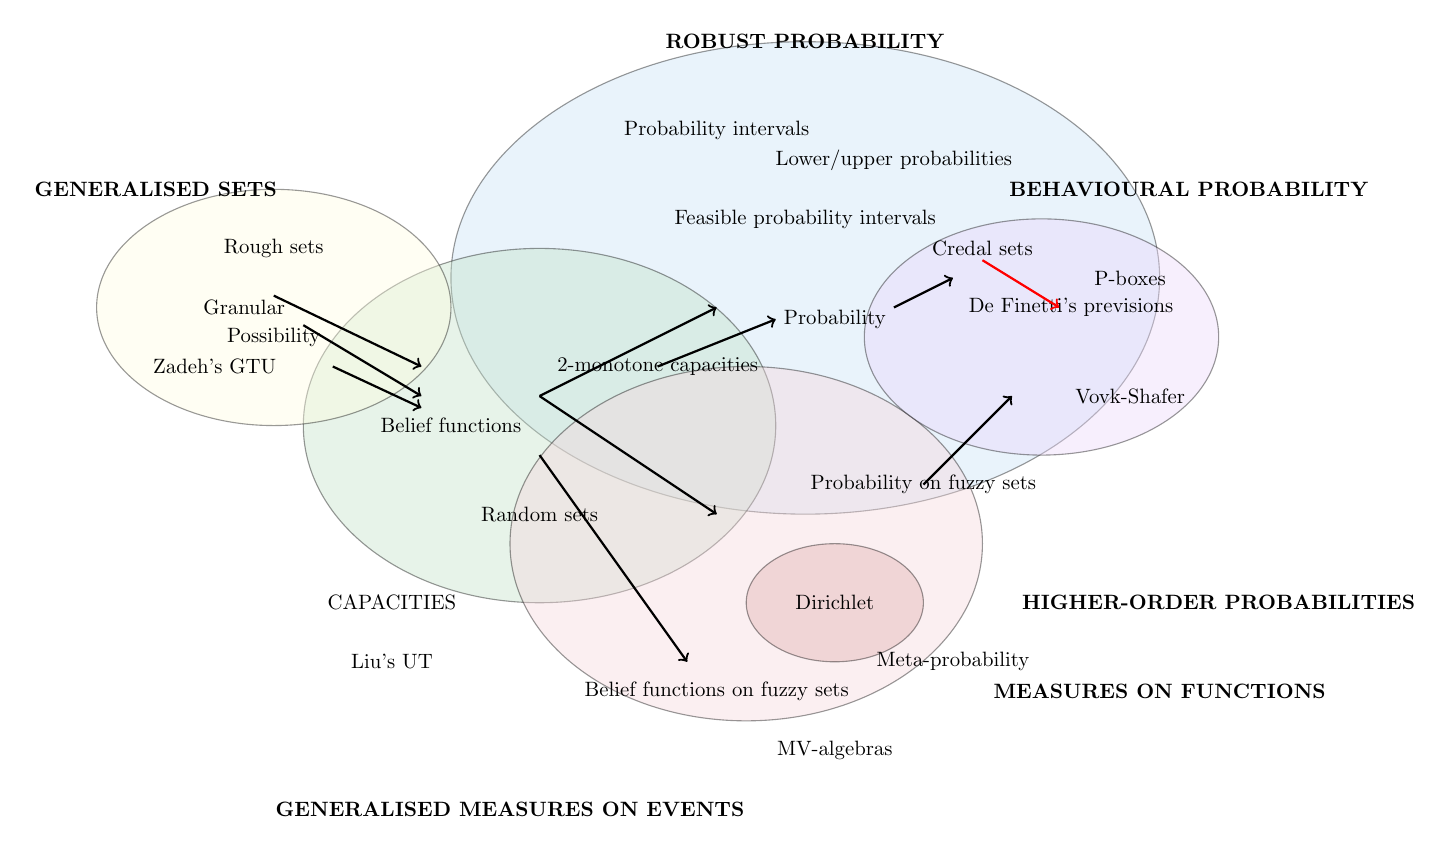
\begin{tikzpicture}[scale=0.75, every node/.style={scale=0.75}]

    % Colors
    \definecolor{bluearea}{RGB}{200,225,245}
    \definecolor{greenarea}{RGB}{195,225,200}
    \definecolor{yellowarea}{RGB}{255,253,225}
    \definecolor{redarea}{RGB}{245,215,220}
    \definecolor{purplearea}{RGB}{235,215,250}
    \definecolor{darkredarea}{RGB}{225,175,175}
    
    % Ellipses
    \draw[fill=bluearea,opacity=.4] (4,4.5) ellipse (6cm and 4cm);
    \draw[fill=greenarea,opacity=.4] (-0.5,2) ellipse (4cm and 3cm);
    \draw[fill=yellowarea,opacity=.4] (-5,4) ellipse (3cm and 2cm);
    \draw[fill=redarea,opacity=.4] (3,0) ellipse (4cm and 3cm);
    \draw[fill=purplearea,opacity=.4] (8,3.5) ellipse (3cm and 2cm);
    \draw[fill=darkredarea,opacity=.4] (4.5,-1) ellipse (1.5cm and 1cm);
    
    % Nodes (Texts)
    % Robust Probability
    \node at (4,8.5) {\textbf{ROBUST PROBABILITY}};
    \node at (2.5,7) {Probability intervals};
    \node at (5.5,6.5) {Lower/upper probabilities};
    \node at (4,5.5) {Feasible probability intervals};
    \node at (7,5) {Credal sets};
    \node at (9.5,4.5) {P-boxes};
    \node at (4.5,3.8) {Probability};
    
    % Generalised Sets
    \node at (-7,6) {\textbf{GENERALISED SETS}};
    \node at (-5,5) {Rough sets};
    \node at (-5.5,4) {Granular};
    \node at (-5,3.5) {Possibility};
    \node at (-6,3) {Zadeh's GTU};
    
    % Capacities
    \node at (-3,-1) {CAPACITIES};
    \node at (-2,2) {Belief functions};
    \node at (-0.5,0.5) {Random sets};
    \node at (-3,-2) {Liu's UT};
    \node at (1.5,3) {2-monotone capacities};
    
    % Behavioural Probability
    \node at (10.5,6) {\textbf{BEHAVIOURAL PROBABILITY}};
    \node at (8.5,4) {De Finetti's previsions};
    \node at (9.5,2.5) {Vovk-Shafer};
    
    % Measures on Functions
    \node at (10,-2.5) {\textbf{MEASURES ON FUNCTIONS}};
    \node at (6,1) {Probability on fuzzy sets};
    \node at (4.5,-1) {Dirichlet};
    \node at (6.5,-2) {Meta-probability};
    \node at (2.5,-2.5) {Belief functions on fuzzy sets};
    \node at (4.5, -3.5) {MV-algebras};
    
    \node at (11,-1) {\textbf{HIGHER-ORDER PROBABILITIES}};
    
    % Generalised measures on events
    \node at (-1,-4.5) {\textbf{GENERALISED MEASURES ON EVENTS}};
    
    % Arrows
    \draw[->,thick] (-4,3) -- (-2.5,2.3);
    \draw[->,thick] (-4.5,3.7) -- (-2.5,2.5);
    \draw[->,thick] (-5,4.2) -- (-2.5,3);
    \draw[->,thick] (-0.5,2.5) -- (2.5,4);
    \draw[->,thick] (-0.5,2.5) -- (2.5,0.5);
    \draw[->,thick] (-0.5,1.5) -- (2,-2);
    \draw[->,thick] (1.5,3) -- (3.5,3.8);
    \draw[->,thick] (5.5,4) -- (6.5,4.5);
    \draw[->,thick] (6,1) -- (7.5,2.5);
    \draw[->,thick,red] (7,4.8) -- (8.3,4);
    
    \end{tikzpicture}

\section{Structure of this work}

This work follows a logical progression from conceptual foundations to a practical application of fuzzy sets. \textbf{Chapter 1} established the context by examining uncertainty and identifying vagueness as a key challenge that traditional frameworks struggle to address, thus motivating the fuzzy paradigm. Building on this foundation, \textbf{Chapter 2} develops the theoretical framework systematically by presenting Fuzzy Set Theory, including its core definitions, operational tools such as t-norms, extensions to fuzzy relations and numbers, as well as briefly introducing the concepts of Possibility distributions and fuzzy propositional logic. \textbf{Chapter 3} explores Multi-Criteria Decision Making (MCDM), detailing methods for converting qualitative information into fuzzy format (fuzzification) and combining multiple criteria into coherent evaluations (aggregation). \textbf{Chapter 4} presents a comprehensive case study of a complex maintenance scheduling problem which leverages fuzzy MCDM concepts and techniques. The \textbf{appendices} contain supplementary technical material regarding analytical properties of t-norms and connections between algebraic structures and fuzzy logic.





